%!TEX root = ../calculus_tutorial.tex

\section*{Overview and a look ahead}

	The goal of this tutorial is to introduce you to the language of calculus.
	The concept maps in Figure~\ref{fig:calculus_tutorial_overview}
	shows a condensed overview of the calculus ideas you'll learn in the next pages.

	\begin{figure}[htb]
		\centering
		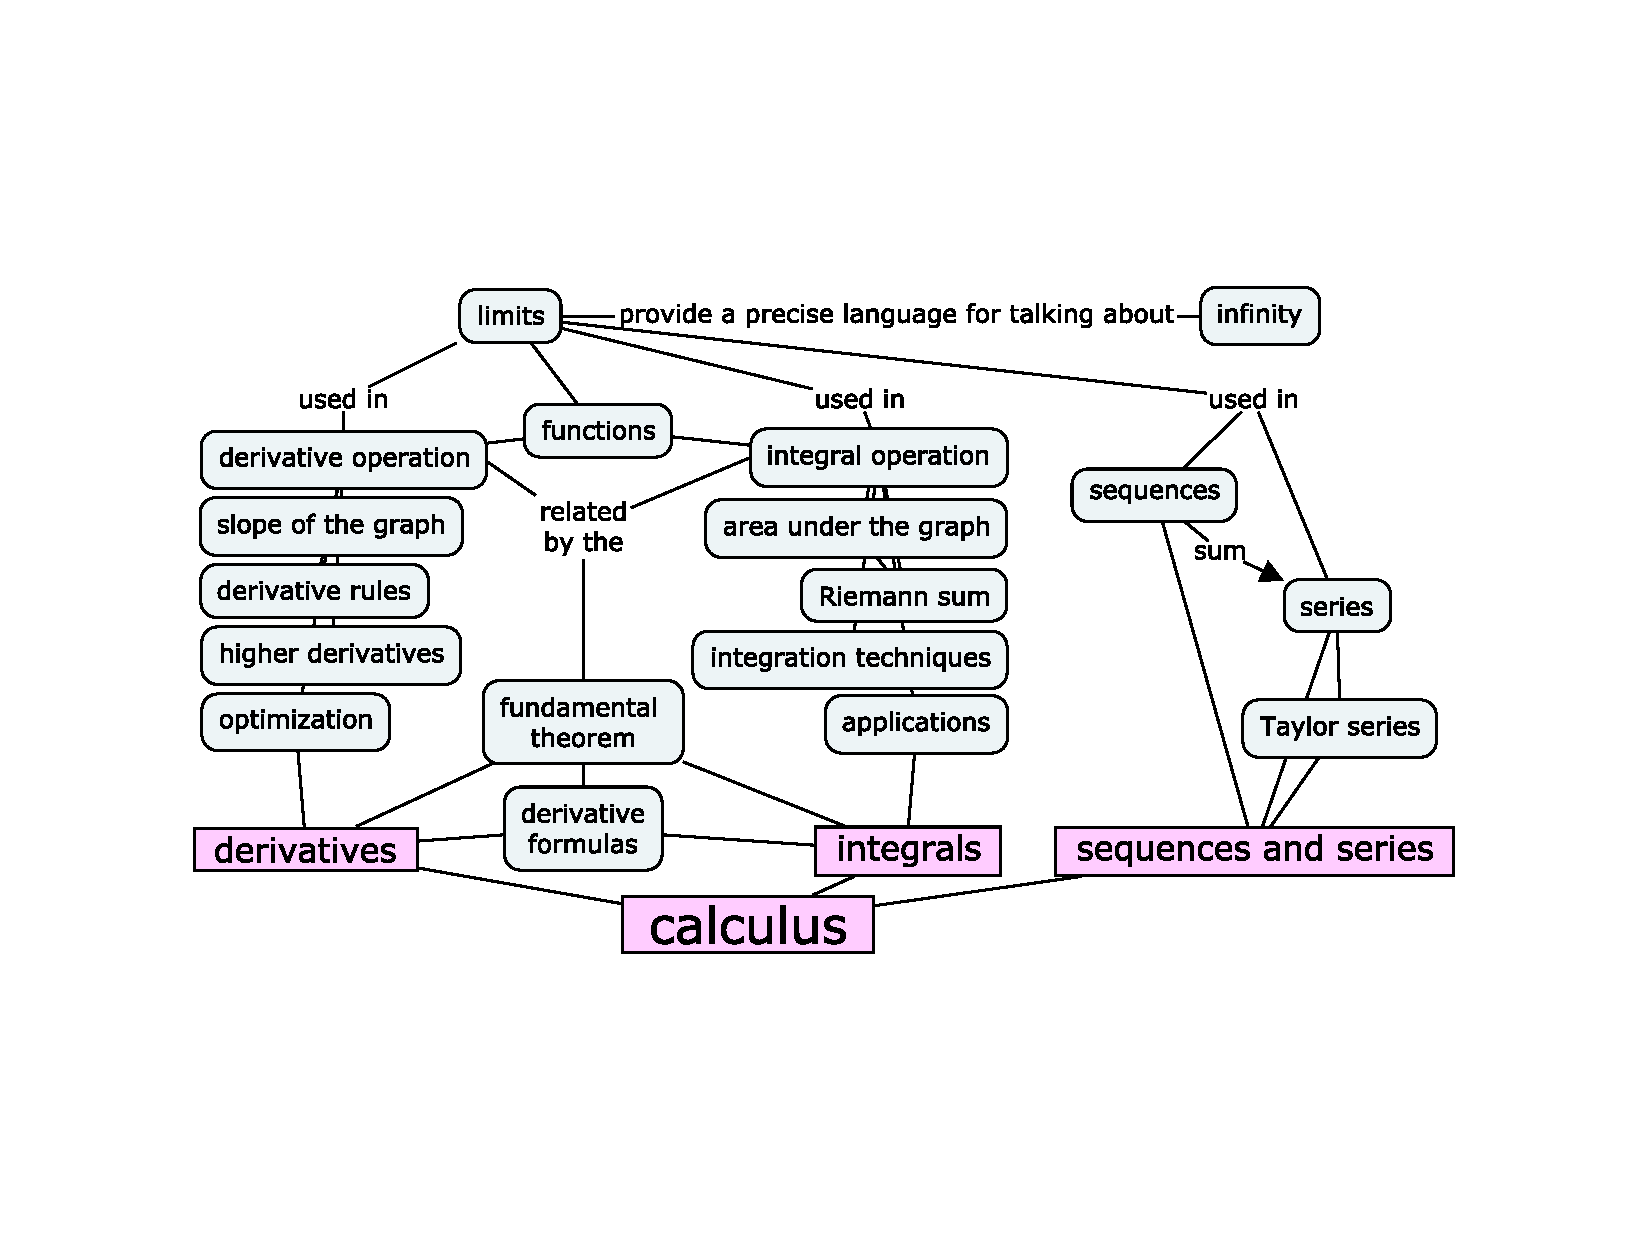
\includegraphics[width=0.99\columnwidth]{figures/calculus/calculus_tutorial_overview.pdf}%
		\vspace{-2mm}
		\caption{	The calculus concepts and topics you'll learn in this tutorial.}
		\label{fig:calculus_tutorial_overview}
	\end{figure}

	We'll start % theis tutorial
	by introducing limits in Section~\ref{sec:limits}
	which provide us with a precise language to talk about infinity.
	% ALT: talk about infinitely large and infinitely small quantities
	Limits are a cornerstone idea in calculus,
	since they allow us to define the calculus operations:
	limits, integrals, and series.
	%
	We'll then discuss derivatives 
	in Section~\ref{sec:derivatives}
	and integrals in Section~\ref{sec:integrals}.
	We'll conclude the tutorial by introducing sequences and series
	in Section~\ref{sec:sequences_and_series}.

	Throughout the tutorial,
	we'll explain concepts using text, formulas, graphs, and code examples.
	My intention is for you to understand the key ideas of calculus in theory,
	but also learn some practical calculation skills you can use to solve real-world problems.

